\documentclass{beamer}

% Style
\usepackage{xcolor}

\usetheme{Madrid}
\usepackage{dirtree}
% Color
\definecolor{flatblue}{RGB}{106, 137, 204}
\usecolortheme[named=flatblue]{structure}
% Font
\usepackage{emoji}
\usepackage{fontspec}
\usepackage{csquotes}
\setsansfont{EB Garamond}
% Code
\usepackage{listings}
\usepackage{graphicx}
\usepackage{hyperref}
\hypersetup{
    colorlinks=true,
    linkcolor=flatblue,
    filecolor=flatblue,
    urlcolor=flatblue,
    citecolor=flatblue
}
\definecolor{flatgreen}{RGB}{0, 98, 102}
\definecolor{flatgreyish}{RGB}{209, 216, 224}
\lstset{
    basicstyle=\ttfamily\scriptsize,
    backgroundcolor=\color{flatgreyish},
    keywordstyle=\color{flatgreen},        % Keywords font ('*' = uppercase)
    commentstyle=\color{flatblue},         % Step between two line-numbers
    columns=fullflexible,
    breaklines=true
}

% Highlight
\usepackage[most]{tcolorbox}
\usepackage{amsmath}
\definecolor{flatorange}{RGB}{255, 165, 2}
\definecolor{flatred}{RGB}{255, 71, 87}
\tcbset{textmarker/.style={%
skin=enhancedmiddle jigsaw,breakable,parbox=false,
boxrule=0mm,leftrule=2mm,rightrule=0mm,boxsep=0mm,arc=0mm,outer arc=0mm,
left=1mm,right=1mm,top=1mm,bottom=1mm,toptitle=1mm,bottomtitle=1mm}}
\newtcolorbox{dangercolorbox}{textmarker,colback=flatorange,colframe=flatred}

% Title
\title{Tests Logiciels - Master MS2D}
\author{Christophe Brun}
\institute{Campus Saint-Michel IT}
\date{21 septembre 2033}
\beamertemplatenavigationsymbolsempty



\titlegraphic{
    \bigbreak
    
\includegraphics[width=2cm]{image/logo-papit.png}
    
\includegraphics[width=2cm]{image/logo-campus-saint-michel-it.png}
}
\begin{document}

    \begin{frame}
        \transdissolve
        \titlepage
    \end{frame}

    \begin{frame}{Table des matières}
        \tableofcontents
    \end{frame}


    \section{Programme du module}
    \begin{frame}
        \frametitle{Tests Logiciels}
        \framesubtitle{Le programme des 3 jours du module}
        \transdissolve
        Compétences :
        \begin{itemize}
            \item Savoir développer et mettre en place des tests unitaires sur une application.

            \item Savoir développer et mettre en place des tests d’intégration sur une application.

            \item Savoir configurer un pipeline d’intégration continue sur une application.

        \end{itemize}
        \centering
        
\includegraphics[width=3cm]{image/funny-cartoon-of-a-smart-young-computer-scientist.png}
    \end{frame}

    \begin{frame}
        \frametitle{Tests Logiciels}
        \framesubtitle{Le programme des 3 jours du module}
        \transdissolve
        Programme :
        \begin{enumerate}
            \item Les tests unitaires
            \begin{itemize}
                \item Qu’est-ce qu’un test ?
                \item Les tests unitaires
                \item Les bonnes pratiques
                \item Le Test Driven Development
                \item Le code coverage
                \item Tests avec langage naturel
            \end{itemize}
            \item  Les tests d’intégration
            \begin{itemize}
                \item  Les tests d’intégration
                \item  Le fonctionnement
                \item  Les bonnes pratiques
            \end{itemize}
            \item L’intégration continue
            \begin{itemize}
                \item  Mise en place d’une plateforme d’intégration continue (GitLab CI)
                \item  Conteneurisation d’une application (API)
                \item  Configuration d’un pipeline de tests
            \end{itemize}
        \end{enumerate}
    \end{frame}

    \begin{frame}
        \transdissolve
        \frametitle{Intervenant sur le module Tests Logiciels}
        \framesubtitle{Christophe Brun, CTO d'In France}

        \begin{columns}
            \column{0.7\textwidth}
            \begin{itemize}
                \item 1\textsuperscript{ere} année d’intervenant à Saint-Michel \emoji{star-struck}.

                \item 7 ans de conseil en développement au sein d’SSII.

                \item 6 ans de conseil en développement à mon compte \href{https://papit.fr}{PapIT}.

                \item Directeur technique et associé d’\href{https://in-france.fr}{In France}.

                \item Passionné !
                \bigbreak
                \begin{columns}
                    \column{0.5\textwidth}
                    \centering
                    
\includegraphics[width=3cm]{image/logo-uppa.png}
                    \column{0.5\textwidth}
                    \centering
                    
\includegraphics[width=3cm]{image/logo-universite-bordeaux.png}
                \end{columns}
            \end{itemize}
            \column{0.3\textwidth}
            \centering
            
\includegraphics[width=5cm]{image/trombine-christophe.jpg}
        \end{columns}
    \end{frame}


    \section{Généralités}
    \begin{frame}
        \frametitle{Qu’est-ce qu’un test ?}
        \framesubtitle{Définition de l'International Software Testing Qualifications Board et IBM}
        \transdissolve
        L’ISTQB définit les termes suivants dans son glossaire\footnote{ISTQB, Glossaire des termes utilisés en tests de logiciels, \url{https://www.cftl.fr/wp-content/uploads/2018/10/Glossaire-des-tests-logiciels-v3_2F-ISTQB-CFTL-1.pdf}} :

        \textbf{Test :} Un ensemble d’un ou plusieurs cas
        de tests.

        \textbf{Cas de test :} Un ensemble de conditions
        préalables, de données d'entrée, d'actions
        (le cas échéant), de résultats attendus et
        de postconditions, élaboré sur la base des
        conditions de test.
        \bigbreak
        Selon IBM\footnote{IBM, Qu'est-ce que le test logiciel ?, \url{https://www.ibm.com/fr-fr/topics/software-testing}} :

        \textquote{Le test logiciel est le processus qui consiste à évaluer et à vérifier qu'un produit ou une application logicielle fait ce qu'il ou elle est censé(e) faire.}
    \end{frame}

    \begin{frame}
        \frametitle{Histoire du test logiciel moderne}
        \transdissolve
        \begin{itemize}
            \item ISTQB, l’International Software Testing Qualifications Board a été fondée en 1998.\footnote{ISTQB, About Us, \url{https://www.istqb.org/about-us/who-we-are}}

            \item Dans son livre Extreme Programming Explained, Kent Beck parle de \textquote{Test-first Programming} en 1999.

            \item Les standards modernes datent de la fin des années 90, début des années 2000.

            \item JUnit, le framework de test le plus utilisé en Java date de 2002.\footnote{Steven J. Zeil, Unit Testing Frameworks, \url{https://www.cs.odu.edu/~zeil/cs350/latest/Public/junit/index.html}}

            \item Début du BDD (Behavior-Driven Development) avec JBehave, censé remplacer JUnit en utilisant le behavior au lieu de test, date de 2023.\footnote{Cucumber, \url{https://cucumber.io/docs/bdd/history/}}
        \end{itemize}
    \end{frame}

    \begin{frame}
        \transdissolve
        \frametitle{La Pyramide des tests}
        \begin{columns}
            \column{0.3\textwidth}
            Différents types de tests peuvent être identifiés.
            La classification la plus classique étant la suivante\footnotemark :
            \column{0.7\textwidth}
            \centering
            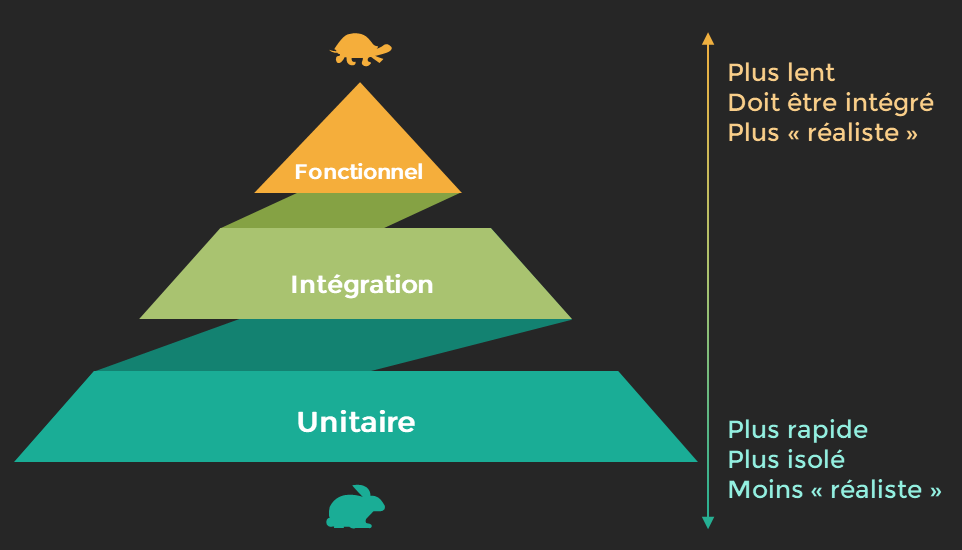
\includegraphics[width=7cm]{image/classic-test-pyramid.png}
        \end{columns}
        \bigbreak
        \footnotetext{OPENCLASSROOMS, Testez votre code Java pour réaliser des applications de qualité, \url{https://openclassrooms.com/fr/courses/6100311-testez-votre-code-java-pour-realiser-des-applications-de-qualite/6616481-decouvrez-les-tests-dintegration-et-les-tests-fonctionnels}}
        Mais d'autres valent le coup d'être découvertes...

    \end{frame}

    \begin{frame}
        \transdissolve
        \frametitle{Brief sur les outils de test logiciel}
        \begin{itemize}
            \item Les frameworks de test retournent 3 statuts, OK, FAILED et ERROR.

            \item OK si aucune erreur n’a lieu et FAILED en cas d’erreur d’assertion, \lstinline{AssertionError} en Python et Java.

            \item Pas de standard universellement accepté mais un format domine, le XML JUnit. Un XML le définit par la grammaire \url{https://windyroad.com.au/dl/Open\%20Source/JUnit.xsd}.

            \item Vient de l’écosystème Java avec le package du même nom, JUnit, mais est présent dans la plupart des frameworks de test comme PHPUnit, Pytest.

            \item L’interopérabilité entre les outils est permise par cette XSD commune, mais pas plus de contrainte. Par exemple, l’interopérabilité entre les frameworks de test et les outils de CI/CD.

            \item Certains outils, souvent des solutions propriétaires, rechignent toujours à exporter un JUnit contenant les résultats de test pour fermer leur environnement.

        \end{itemize}
    \end{frame}


    \begin{frame}[fragile]
        \frametitle{L'assertion error}
        \framesubtitle{En Python}
        \transdissolve
        L’instruction \lstinline{assert} vérifie une condition.
        Si la condition est vraie, cela ne fait rien et votre programme continue simplement à s’exécuter. Mais si la condition d’assertion est fausse, elle lève une exception \lstinline{AssertionError}.
        \begin{lstlisting}[language=Python]
assert 23 % 2 == 0, "Le restant de la division est différent de 0"
        \end{lstlisting}
        Étant toujours fausse, le programme crash.
        \begin{lstlisting}[language=sh]
chrichri@chrichri-HKD-WXX:~$ python3 -c 'assert 23 % 2 == 0, "Le restant de la division est différent de 0"'
Traceback (most recent call last):
  File "<string>", line 1, in <module>
AssertionError: Le restant de la division est différent de 0
        \end{lstlisting}
    \end{frame}


    \section{Pytest}
    \begin{frame}
        \frametitle{Pourquoi Pytest pour le testing}
        \transdissolve
        \textquote{pytest is a mature full-featured Python testing tool that helps you write better programs.\footnote{pytest: helps you write better programs , \url{https://docs.pytest.org}}}
        \begin{columns}
            \column{0.6\textwidth}
            Pytest est le framework de test en Python le plus utilisé selon les sondages de JetBrains\footnotemark.

            Seuls JUnit et Pytest sont pour tous usages, les autres sont orientés web.
            \column{0.4\textwidth}
            \centering
            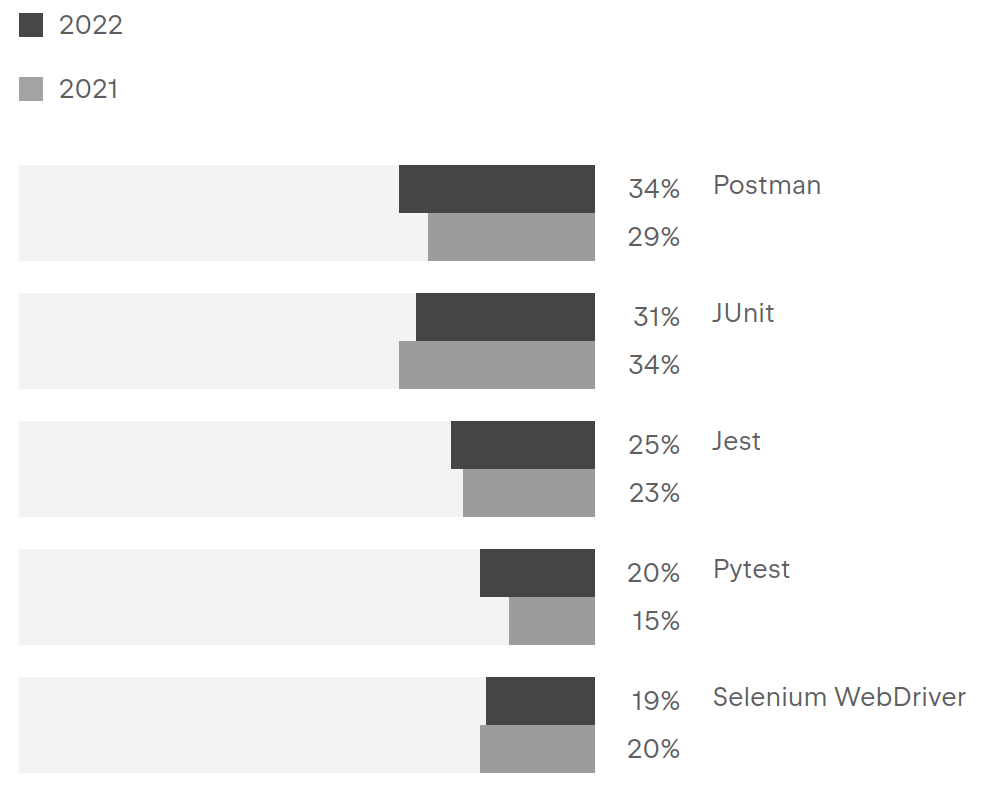
\includegraphics[width=5cm]{image/jetbrains-survey-testing-framework.png}
        \end{columns}
        \footnotetext{JetBrains, Which test frameworks , \url{https://www.jetbrains.com/lp/devecosystem-2022/testing/}}

    \end{frame}

    \begin{frame}[fragile]
        \frametitle{Pytest}
        \framesubtitle{Rédiger un test}
        \transdissolve
        \begin{itemize}
            \item Un module de test Pytest est un module Python préfixé par \lstinline{test_}.

            \item Toutes les méthodes préfixées par \lstinline{test_} sont exécutées par Pytest. Qu'elles soient
            dans une classe ou non. Les autres méthodes ne sont pas exécutées sauf si les tests ne les appellent.
        \end{itemize}
        Ici par exemple, la précédente assertion est intégrées dans une méthode nommée \lstinline{test_divide} dans le module de test \lstinline{test_division.py}.
        \begin{lstlisting}[language=Python]
def test_divide():  # Un test Pytest est préfixé par test_
    assert 23 % 2 == 0, "Le restant de la division est différent de 0."
        \end{lstlisting}
    \end{frame}


    \begin{frame}[fragile]
        \frametitle{Pytest}
        \framesubtitle{Lancer les tests}
        \transdissolve
        Lancer avec la commande \lstinline{python -m pytest test_divison.py}, Pytest affiche le rapport de test.
        \begin{lstlisting}[language=sh]
...
def test_divide():  # Un test Pytest est préfixé par test_
>       assert 23 % 2 == 0, "Le restant de la division est différent de 0."
E       AssertionError: Le restant de la division est différent de 0.
E       assert (23 % 2) == 0

test_divison.py:2: AssertionError
...
        \end{lstlisting}

        De très utiles et nombreuses options peuvent compléter cette ligne de commande.
        Pour les découvrir, lancez \lstinline{python -m pytest --help} et \textquote{RTFM}.
    \end{frame}

    \begin{frame}[fragile]
        \frametitle{Pytest}
        \framesubtitle{Les tests paramétriques}
        \transdissolve
        Les tests paramétriques sont des tests qui prennent un ensemble de paramètres en entrées.

        Ils permettent de tester plusieurs cas avec un seul test.

        Le rapport génère un cas de test par paramètre. Il est donc plus détaillé et permet de trouvé
        les tests en échec plus facilement que si l'\lstinline {assert} était dans une boucle, ce qui ne donne qu'un statut OK ou Fail dans le rapport.
        \begin{lstlisting}[language=Python]
import pytest
...
@pytest.mark.parametrize("dividend", range(100))  # Paramétrage du test
def test_divide_from_0_to_99(dividend):  # Doit avoir un argument présent dans le paramétrage
    assert dividend % 2 == 0, "Le restant de la division est différent de 0."
        \end{lstlisting}
    \end{frame}

    \begin{frame}[fragile]
        \frametitle{Pytest}
        \framesubtitle{Les tests paramétriques}
        \transdissolve
        Génère 100 cas de tests. Met en évidence les dividendes dont le restant de la division par 2 est différent de 0, ici 1 par exemple.
        \begin{lstlisting}[language=sh]
collecting ... collected 100 items

test_divison.py::test_divide_from_0_to_99[0] PASSED                      [  1%]
test_divison.py::test_divide_from_0_to_99[1] FAILED                      [  2%]
test_divison.py:7 (test_divide_from_0_to_99[1])
1 != 0

Expected :0
Actual   :1
<Click to see difference>

dividend = 1

    @pytest.mark.parametrize("dividend", range(100))  # Paramétrage du test
    def test_divide_from_0_to_99(dividend):  # Doit avoir un argument présent dans le paramétrage
>       assert dividend % 2 == 0, "Le restant de la division est différent de 0."
E       AssertionError: Le restant de la division est différent de 0.
E       assert (1 % 2) == 0
        \end{lstlisting}
    \end{frame}

    \begin{frame}[fragile]
        \frametitle{Pytest}
        \framesubtitle{Plantage dans un test, quel statut?}
        \transdissolve
        Ce test crash avant l'assert.
        \begin{lstlisting}[language=Python]
def test_fail_or_error():  # Une erreur donne un fail ou error?
    dividende = 23 / 0
    assert dividende % 2 == 0, \
        "Le restant de la division est différent de 0."
        \end{lstlisting}
        Malgré l'absence d'\lstinline{assertionError}, le test est en échec et non en erreur.
        \begin{lstlisting}[language=sh]
test_divison.py::test_fail_or_error FAILED                               [100%]
test_divison.py:12 (test_fail_or_error)
def test_fail_or_error():  # Une erreur donne un fail ou error?
>       dividende = 23 / 0
E       ZeroDivisionError: division by zero

test_divison.py:14: ZeroDivisionError
        \end{lstlisting}

        \begin{dangercolorbox}
            Pour éviter les faux négatifs, un test doit tendre, tant que faire se peut, vers un \lstinline{assert}. Pour cela pensez à utiliser les fonctions \lstinline{parametrize} et \lstinline{fixture}.
        \end{dangercolorbox}
    \end{frame}

    \begin{frame}[fragile]
        \frametitle{Pytest}
        \framesubtitle{Les fixtures}
        \transdissolve
        Cf. \url{https://github.com/St-Michel-IT/testing/blob/main/test_customer_database.py}

        Un \lstinline{return} ou un \lstinline{yield} envoie l'objet au test dans l'état voulu.
        \begin{lstlisting}[language=Python]
def customer_without_table():
    """...
    """
    customer = Customer()  # Avant le test, c'est le setup
    yield customer  # Un yield évite de sortir de la fonction
    customer.con.close()  # Après le test, le teardown
        \end{lstlisting}
        Le test n'a qu'une seule ligne, qu'un \lstinline{assert} l'échec ne
        pourrait venir que de là.
        \begin{lstlisting}[language=Python]
def test_instantiation(customer_without_table):
    """...
    """
    assert isinstance(customer_without_table.con, Connection)
        \end{lstlisting}
        En cas de plantage dans la fixture, i.e. avant ou après le test, la sanction
        serait erreur et non échec.

        Le rapport reflétera fidèlement le test et sera exempt de faux négatif.
    \end{frame}

    \begin{frame}[fragile]
        \frametitle{Pytest}
        \framesubtitle{Le scope des fixtures}
        \transdissolve
        L'argument \lstinline{scope} du décorateur \lstinline{pytest.fixture} défini la durée de vie
        de la fixture. Il peut prendre 3 valeurs :
        \begin{itemize}
            \item \lstinline{function} : La valeur par défaut si on ne met rien.
            La fixture est exécutée à chaque fonction de test \lstinline{def test_...} qui l'appelle directement ou indirectement, donc les éventuels setup et teardown de cette dernière aussi.
            \item \lstinline{module} : Une fois par module \lstinline{test_....py}.
            \item \lstinline{session} : Une seule fois durant la session de test quel que soit le nombre de modules et de tests exécutés.
        \end{itemize}
        \begin{lstlisting}[language=Python]
@pytest.fixture(scope="function")  # Scope de la fixture, par default function
def customer_without_table():
    """
    Connection to in memory database using the Customer class
        \end{lstlisting}

        Pour tester une API en étant sûr le token n'est pas périmé, on peut utiliser le scope \lstinline{function} pour en avoir un nouveau à chaque appel.

        Si préparer les conditions initiales, le setup, prend du temps, on évitera si possible de se répéter à chaque test avec les scopes \lstinline{module} \lstinline{session}.
    \end{frame}

    \begin{frame}
        \frametitle{Pytest}
        \framesubtitle{\lstinline{Le conftest.py}}
        \transdissolve
        Il n'a qu'une seule particularité, c'est d'être importé automatiquement par Pytest lorsqu'il est présent dans le dossier courant des tests.

        Il permet de factoriser les fixtures et les paramétrages de tests utilisés dans plusieurs modules de tests, car ces derniers seront automatiquement disponible sans même un import dans le module.
        \begin{columns}
            \column{0.5\textwidth}
            \dirtree{%
                .1 ./.
                .2 {conftest.py}.
                .2 {\textcolor{flatgreen}{test\_no\_directory.py}}.
                .2 unit.
                .3 {\textcolor{flatgreen}{test\_integration.py}}.
                .2 functional.
                .3 {\textcolor{flatgreen}{test\_functional.py}}.
            }\column
            {0.5\textwidth}
            Pour tous ces tests, s'ils sont lancés depuis la racine avec la commande \lstinline{pytest}, le \lstinline{conftest.py} sera importé automatiquement.
        \end{columns}
        \bigbreak
        \begin{columns}
            \column{0.9\textwidth}
            PyCharm intègre par défaut Pytest comme lanceur de tests et fournit l'autocomplétion pour les fixtures du \lstinline{conftest.py}.
            \column{0.1\textwidth}
            \centering
            
\includegraphics[width=1cm]{image/logo-pycharm.png}
        \end{columns}
    \end{frame}

    \begin{frame}[fragile]
        \frametitle{Pytest}
        \framesubtitle{Le coverage}
        \transdissolve
        Pas de support natif du coverage par Pytest, il faut installer le plugin \lstinline{pytest-cov}\footnote{Welcome to pytest-cov’s documentation!, \url{https://pytest-cov.readthedocs.io/en/latest/}}.

        Pour appeler le plugin, il faut passe en argument le module à tester et le(s) test(s) de ce dernier.


        \begin{lstlisting}[language=sh]
pytest --cov=\textcolor{flatgreen}{customer_database} ./test_customer_database.py
...
rootdir: /home/chrichri/Documents/Campus-St-Michel-IT/testing
plugins: cov-4.1.0
collected 6 items

test_customer_database.py ......                                                                                                                                                                                                 [100%]

---------- coverage: platform linux, python 3.11.4-final-0 -----------
Name                   Stmts   Miss  Cover
------------------------------------------
customer_database.py       9      0   100%
------------------------------------------
TOTAL                      9      0   100%
        \end{lstlisting}

    \end{frame}

    \begin{frame}
        \frametitle{Pytest}
        \framesubtitle{Le coverage}
        \transdissolve
        \begin{columns}

            \column{0.5\textwidth}
            \centering
            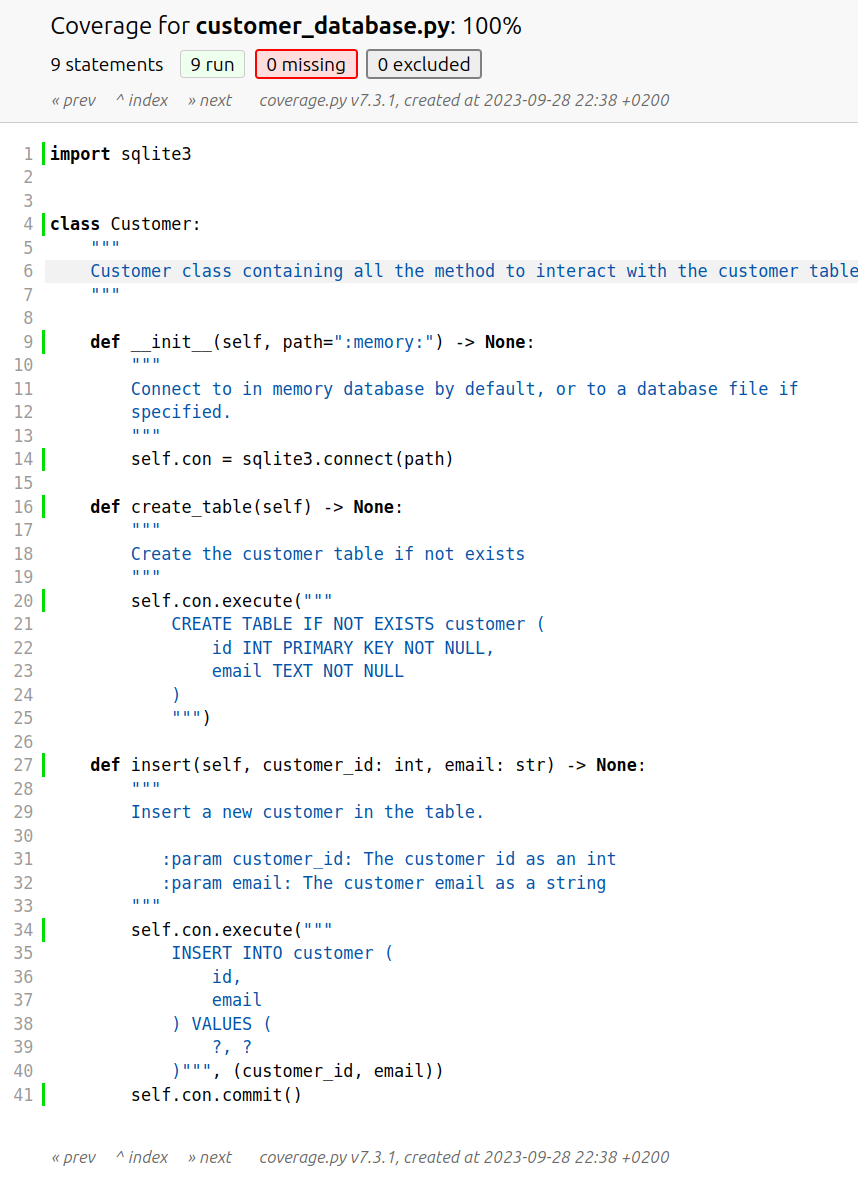
\includegraphics[width=5cm]{image/html-coverage.png}
            \column{0.5\textwidth}
            L'option \lstinline{--cov-report=html} permet de générer un rapport HTML plus détaillé qui met en lumière quelles parties du code sont couvertes par les tests et lesquelles ne le sont pas.
            \bigbreak
            \textbf{Exercice} : Trouvez quel test du module \url{https://github.com/St-Michel-IT/testing/blob/main/test_customer_database.py} couvre quelle partie de ce code:
        \end{columns}

    \end{frame}

    \begin{frame}
        \frametitle{Pytest}
        \framesubtitle{Le secret de la réussite}
        \transdissolve
        \begin{columns}
            \column{0.7\textwidth}
            Pytest est un framework complet voir complexe.

            Mais quasi toutes les fonctionnalités auxquelles on peut penser sont déjà implémentées et décrites une documentation de qualité.

            Comme avec toutes les grosses libraries, il faut avoir confiance en leur design et chercher dedans avant de réinventer la roue.

            La liste des fonctionnalités est trop longue, nous venons juste d'en découvrir les principales.
            \bigbreak
            Donc une fois encore, comme pour toutes les bonnes libraires à connaître, le secret est \textquote{\textbf{\Large{RTFM}}} !
            \column{0.3\textwidth}
            \centering
            
\includegraphics[width=3cm]{image/girl-rtfm.png}
        \end{columns}

    \end{frame}

    \begin{frame}
        \frametitle{Pytest}
        \framesubtitle{Travaux dirigés sur les tests unitaires}
        \transdissolve
        Les tests unitaires peuvent-être défini comme ceux testant les classes et fonctions d'une seule librairie.

        Exemple de la librairie du repo \url{https://github.com/St-Michel-IT/testing/}, le module \lstinline{customer_database.py} testé par \lstinline{test_customer_database.py} est donc un exemple de tests unitaires.
        \bigbreak
        \textbf{Exercice} : Toujours dans le même repo, le module \lstinline{witness_number.py} est un début implémentation d'une généralisation du petit théorème de Fermat expliquée sur la chaîne Youtube Numberphile par Matt Parker\footnote{Numberphile, Witness Numbers (and the truthful 1,662,803), \url{https://www.youtube.com/watch?v=_MscGSN5J6o}}.
        Cette librairie n'est pas déjà libre sur le web, finissons son développement avec des standards de qualité élevés grâce à nos connaissances en testing.
    \end{frame}

\end{document}
